% A1 landscape poster (841 x 594 mm) for the Research Paper Auditor final report.
% Build: pdflatex poster_landscape.tex
\documentclass{article}
\usepackage[paperwidth=841mm,paperheight=594mm,margin=10mm]{geometry}
\usepackage[T1]{fontenc}
\usepackage[scaled=0.95]{helvet}
\renewcommand{\familydefault}{\sfdefault}
\renewcommand{\ttdefault}{lmtt}
\usepackage{anyfontsize}
\usepackage{sfmath}
\usepackage{graphicx}
\usepackage{xcolor}
\usepackage{fontawesome5}
\usepackage[most]{tcolorbox}
\usepackage{pgfplots}
\usetikzlibrary{arrows.meta}
\pgfplotsset{compat=1.18}
\usepackage{qrcode}
\usepackage{eso-pic}
\usepackage{etoolbox}
\AtBeginEnvironment{minipage}{\raggedright}
\pagestyle{empty}
\setlength{\parindent}{0pt}
\setlength{\parskip}{0pt}
\hyphenpenalty=10000\exhyphenpenalty=10000

% ---- links shown as QR codes
\newcommand{\codeurl}{https://github.com/itikelabhaskar/Research_Paper_auditor}
\newcommand{\websiteurl}{https://va24d.github.io/Research_Paper_auditor/}

% ---- currency
\newcommand{\rs}{\raisebox{0.03em}{\scalebox{0.78}{\faRupeeSign}}\hspace{0.05em}}

% ---- colours matching report and poster
\definecolor{ink}{HTML}{14213D}
\definecolor{blue}{HTML}{0B5CAD}
\definecolor{rulegrey}{HTML}{C9CED6}
\definecolor{cfull}{HTML}{1F6FB2}
\definecolor{cnover}{HTML}{8DBBE3}
\definecolor{cbzero}{HTML}{E08A2E}
\definecolor{cbone}{HTML}{B5443A}
\definecolor{crev}{HTML}{F2C14E}
\definecolor{good}{HTML}{2E7D4F}
\definecolor{bad}{HTML}{C0392B}
\definecolor{hilite}{HTML}{FFE066}
\definecolor{codebg}{HTML}{1E2329}

% ---- type sizes
\newcommand{\body}{\fontsize{18}{22.5}\selectfont}
\newcommand{\smalltext}{\fontsize{15}{18.5}\selectfont}
\newcommand{\hb}[1]{\textbf{\color{blue}#1}}
\newcommand{\hlmark}[1]{\tikz[baseline=(m.base)]\node[fill=hilite, inner xsep=1.2mm, inner ysep=0.8mm, outer sep=0pt](m){\strut\textbf{#1}};}

% ---- section heading
\newcommand{\snum}[1]{\tikz[baseline=(n.base)]\node[circle, fill=blue, text=white, minimum size=10mm,
  inner sep=0pt, font=\sffamily\bfseries\fontsize{20}{20}\selectfont](n){#1};\hspace{3mm}}

\newcommand{\sect}[2]{%
  \parbox[c][13mm][c]{\linewidth}{\snum{#1}\fontsize{23}{27}\selectfont\bfseries\color{ink}#2}\par
  {\color{blue}\rule{\linewidth}{1.0mm}}\par\vspace{3mm}\raggedright}

% ---- comparison bars
\newcommand{\cbar}[4]{%
  \makebox[44mm][l]{#1}\tikz[baseline=-0.6ex]{\fill[#4] (0,-2.5mm) rectangle (#3*36mm,2.5mm);
  \node[anchor=west, font=\bfseries] at (#3*36mm,0) {#2};}\par\vspace{1.5mm}}

% ---- page border
\AddToShipoutPictureBG{%
  \put(0,0){
\begin{tikzpicture}[x=1mm,y=1mm]
    \fill[white] (0,0) rectangle (841,594);
    \draw[blue,line width=3.5mm] (5,5) rectangle (836,589);
  \end{tikzpicture}}}

% ---- headline number
\newcommand{\stat}[4]{%
  \begin{minipage}[t]{\linewidth}\centering
  {\fontsize{48}{52}\selectfont\bfseries\color{#1}#2}\\[1.5mm]
  {\fontsize{19}{23}\selectfont\bfseries\color{ink}#3}\\[1mm]
  {\fontsize{15}{18}\selectfont\color{black!60}#4}
  \end{minipage}}

\pgfplotsset{poster/.style={font=\sffamily\fontsize{15}{18}\selectfont,
  every axis label/.append style={font=\fontsize{16}{20}\selectfont},
  every tick label/.append style={font=\fontsize{15}{18}\selectfont},
  major tick length=2.0mm, axis line style={line width=0.8pt, black!60},
  tick style={black!60}, grid style={black!12,line width=0.6pt},
  xticklabel style={text height=1.7ex, text depth=0.5ex}}}

% ---- section panel box
\newenvironment{col}[2]{\begin{minipage}[t]{#1}\begin{tcolorbox}[enhanced, colback=white,
  colframe=blue!55!ink, boxrule=0.8mm, arc=0mm, left=6mm, right=6mm, top=0mm, bottom=4mm,
  before skip=0pt, after skip=0pt, equal height group=#2]\raggedright}{\end{tcolorbox}\end{minipage}}

\begin{document}
\body\raggedright

% ================================================================ HEADER
\begin{minipage}[c]{56mm}
  
\includegraphics[width=54mm]{../logo.png}
\end{minipage}\hspace{6mm}%
\begin{minipage}[c]{\dimexpr\linewidth-240mm\relax}\raggedright
  {\fontsize{50}{56}\selectfont\bfseries\color{ink}Research Paper Auditor}\\[2.5mm]
  {\fontsize{24}{29}\selectfont\color{blue} Does the paper match its citations and its code?  Evidence-Gated Verification}\\[3mm]
  {\fontsize{21}{25}\selectfont\color{ink} Vijay Aravynthan \quad Itikela Bhaskar \quad Anurag Peddi \quad Sudheera Y S}\\[2.5mm]
  {\fontsize{17}{21}\selectfont\color{black!75}\textbf{SERC} (Software Engineering Research Center) \ \& \ \textbf{CVIT} (Centre for Visual Information Technology)\\
  International Institute of Information Technology, Hyderabad (IIIT-H) \ \textbullet\ \ CL3.410 LMA Final Project}
\end{minipage}\hfill
\begin{minipage}[c]{168mm}
\begin{tcolorbox}[enhanced, colback=blue, colframe=blue, arc=0mm, boxrule=0mm, halign=center,
  left=5mm, right=5mm, top=4mm, bottom=4mm, before skip=0pt, after skip=0pt]
  {\fontsize{18}{22}\selectfont\color{white!85!blue} Labs: \textbf{SERC} \& \textbf{CVIT}\par}\vspace{1mm}
  {\fontsize{34}{40}\selectfont\bfseries\color{white} Hood Research\\Department\par}\vspace{1mm}
  {\fontsize{16}{20}\selectfont\color{white!85!blue} IIIT Hyderabad\par}
\end{tcolorbox}
\end{minipage}

\vspace{3mm}
{\color{ink}\rule{\linewidth}{1.6mm}}

\vspace{3mm plus 1fill}

% ================================================================ ROW 1: Problem | System Pipeline
\begin{col}{0.375\linewidth}{r1}
\sect{1}{The paper says one thing. Its code does another.}
{\centering\resizebox{0.98\linewidth}{!}{%
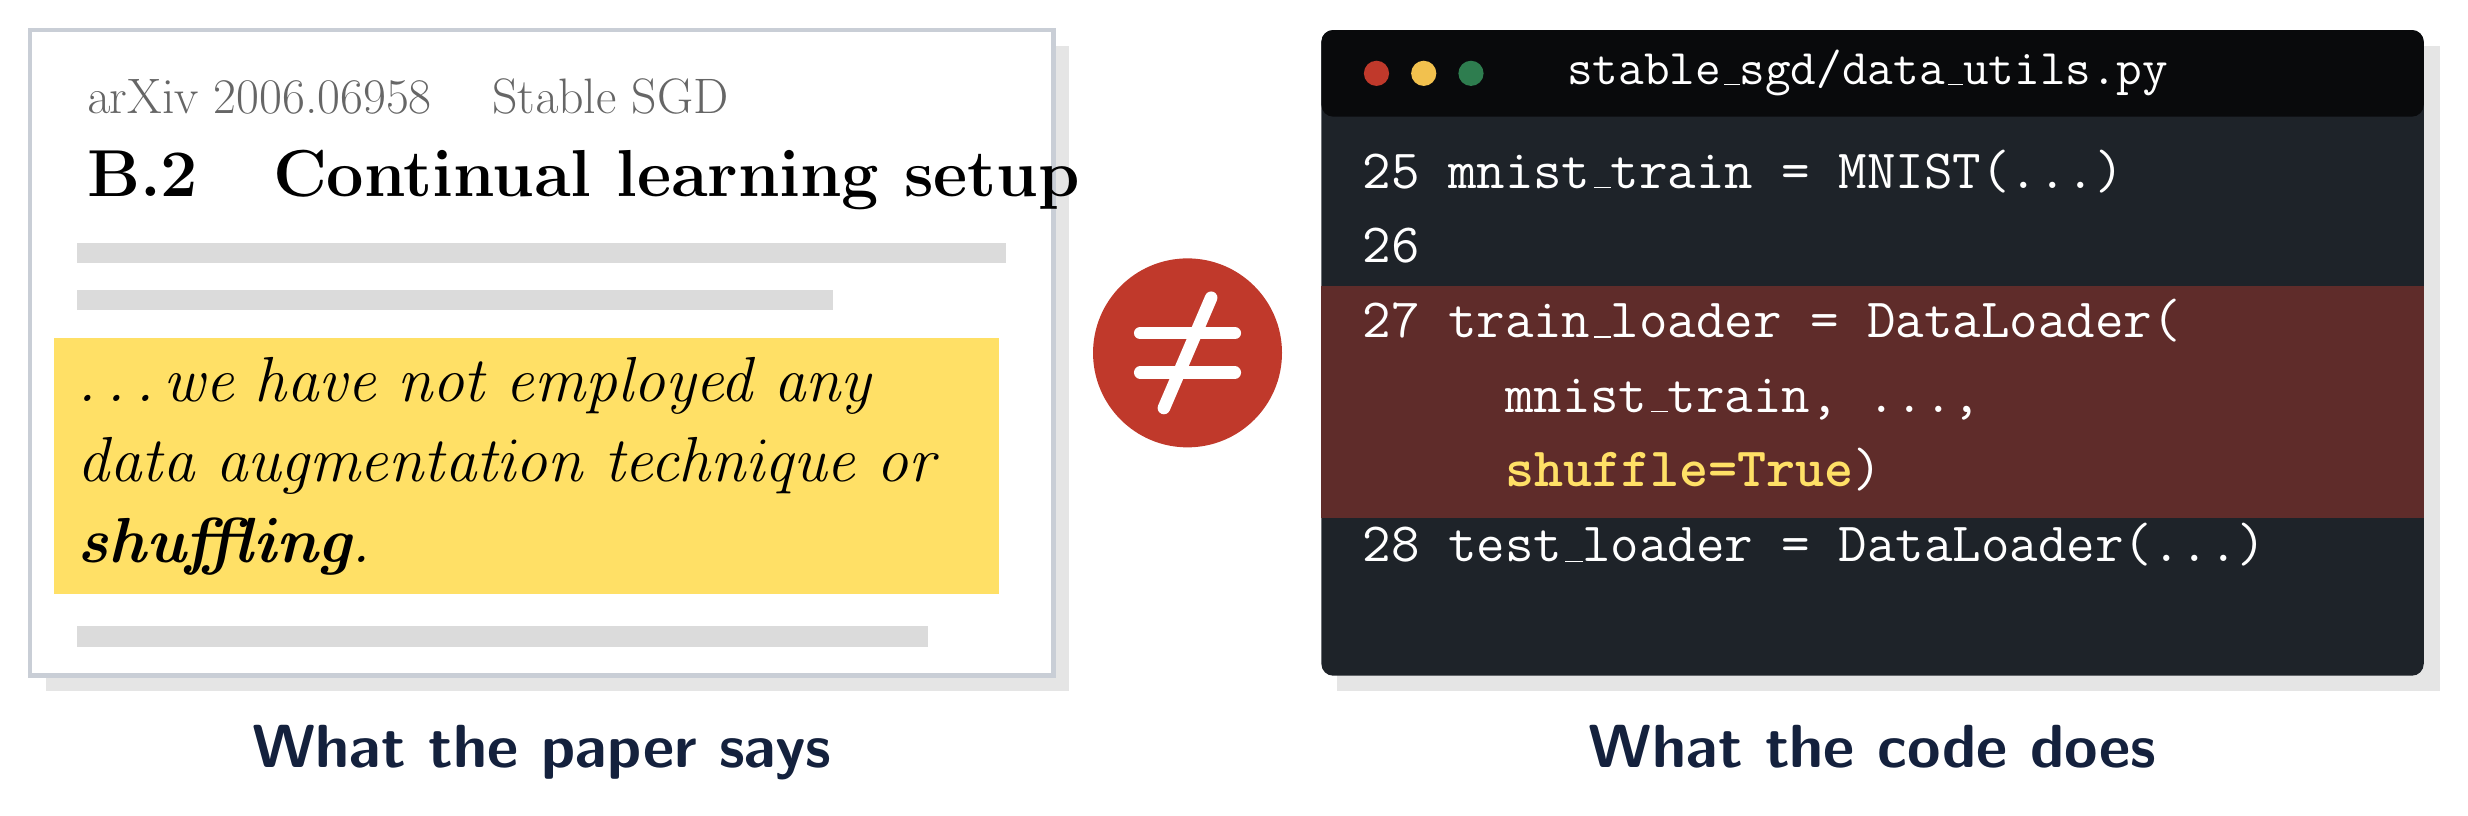
\begin{tikzpicture}[x=1mm,y=1mm]
  \fill[black!10] (2,-2) rectangle (132,-84);
  \draw[rulegrey, line width=0.6mm, fill=white] (0,0) rectangle (130,-82);
  \node[anchor=north west, font=\fontsize{18}{22}\selectfont\rmfamily\color{black!60}] at (6,-5) {arXiv 2006.06958 \quad Stable SGD};
  \node[anchor=north west, font=\fontsize{24}{28}\selectfont\rmfamily\bfseries] at (6,-14) {B.2\quad Continual learning setup};
  \foreach \y/\w in {-27/118,-33/96} \fill[black!14] (6,\y) rectangle (6+\w,\y-2.6);
  \node[anchor=north west, fill=hilite, text width=114mm, inner xsep=3mm, inner ysep=2.5mm,
    font=\fontsize{23}{29}\selectfont\rmfamily\itshape] (quote) at (3,-39)
    {\ldots we have not employed any data augmentation technique or \textbf{shuffling}.};
  \fill[black!14] ([yshift=-4mm]quote.south west -| 6,0) rectangle ++(108,-2.6);
  \fill[bad] (147,-41) circle (12);
  \draw[white, line width=1.6mm, line cap=round] (141,-38.5) -- (153,-38.5) (141,-43.5) -- (153,-43.5);
  \draw[white, line width=1.6mm, line cap=round] (144,-48) -- (150,-34);
  \fill[black!10] (166,-2) rectangle (306,-84);
  \fill[codebg, rounded corners=1.5mm] (164,0) rectangle (304,-82);
  \fill[black!70!codebg, rounded corners=1.5mm] (164,0) rectangle (304,-11);
  \foreach \i/\c in {0/bad,1/crev,2/good} \fill[\c] (171+\i*6,-5.5) circle (1.6);
  \node[anchor=west, font=\fontsize{18}{22}\selectfont\ttfamily\color{white!80}] at (194,-5.5) {stable\_sgd/data\_utils.py};
  \fill[bad!40!codebg] (164,-32.5) rectangle (304,-62);
  \node[anchor=north west, align=left, font=\fontsize{20}{27}\selectfont\ttfamily\color{white!90}] at (168,-14)
    {{\color{white!45}25}\ mnist\_train = MNIST(\ldots)\\
     {\color{white!45}26}\ \\
     {\color{white!45}27}\ train\_loader = DataLoader(\\
     {\color{white!45}\phantom{27}}\ \ \ mnist\_train, \ldots,\\
     {\color{white!45}\phantom{27}}\ \ \ \textbf{\color{hilite}shuffle=True})\\
     {\color{white!45}28}\ test\_loader = DataLoader(\ldots)};
  \node[anchor=north, font=\fontsize{22}{26}\selectfont\bfseries\color{ink}] at (65,-87) {What the paper says};
  \node[anchor=north, font=\fontsize{22}{26}\selectfont\bfseries\color{ink}] at (234,-87) {What the code does};
\end{tikzpicture}}\par}

\vspace{3mm}
\textbf{Real Discovery:} \hlmark{Mirzadeh et al., NeurIPS 2020.} An unlabelled mismatch discovered automatically in an accepted paper. Paper claimed no shuffling; repository sets \texttt{shuffle=True}. Both lines quoted verbatim without human guidance.\\[2mm]
\textbf{The Reviewer Bottleneck:} ICLR received \textbf{62,000+} submissions. Reviewers have minutes per paper and cannot inspect repos or verify cited text. Unaudited claims slip through peer review at scale.
\end{col}\hfill
\begin{col}{0.61\linewidth}{r1}
\sect{2}{Our system: Modular Evidence-Gated Architecture}
Give it a paper and its repository. It \textbf{reports a problem only when it can quote both sides}.\\[1mm]
\hlmark{New:} one automated run inspects citations, claims, static code ASTs, and numbers. Earlier tools check one.

\vspace{2mm}
{\centering\resizebox{\linewidth}{!}{%
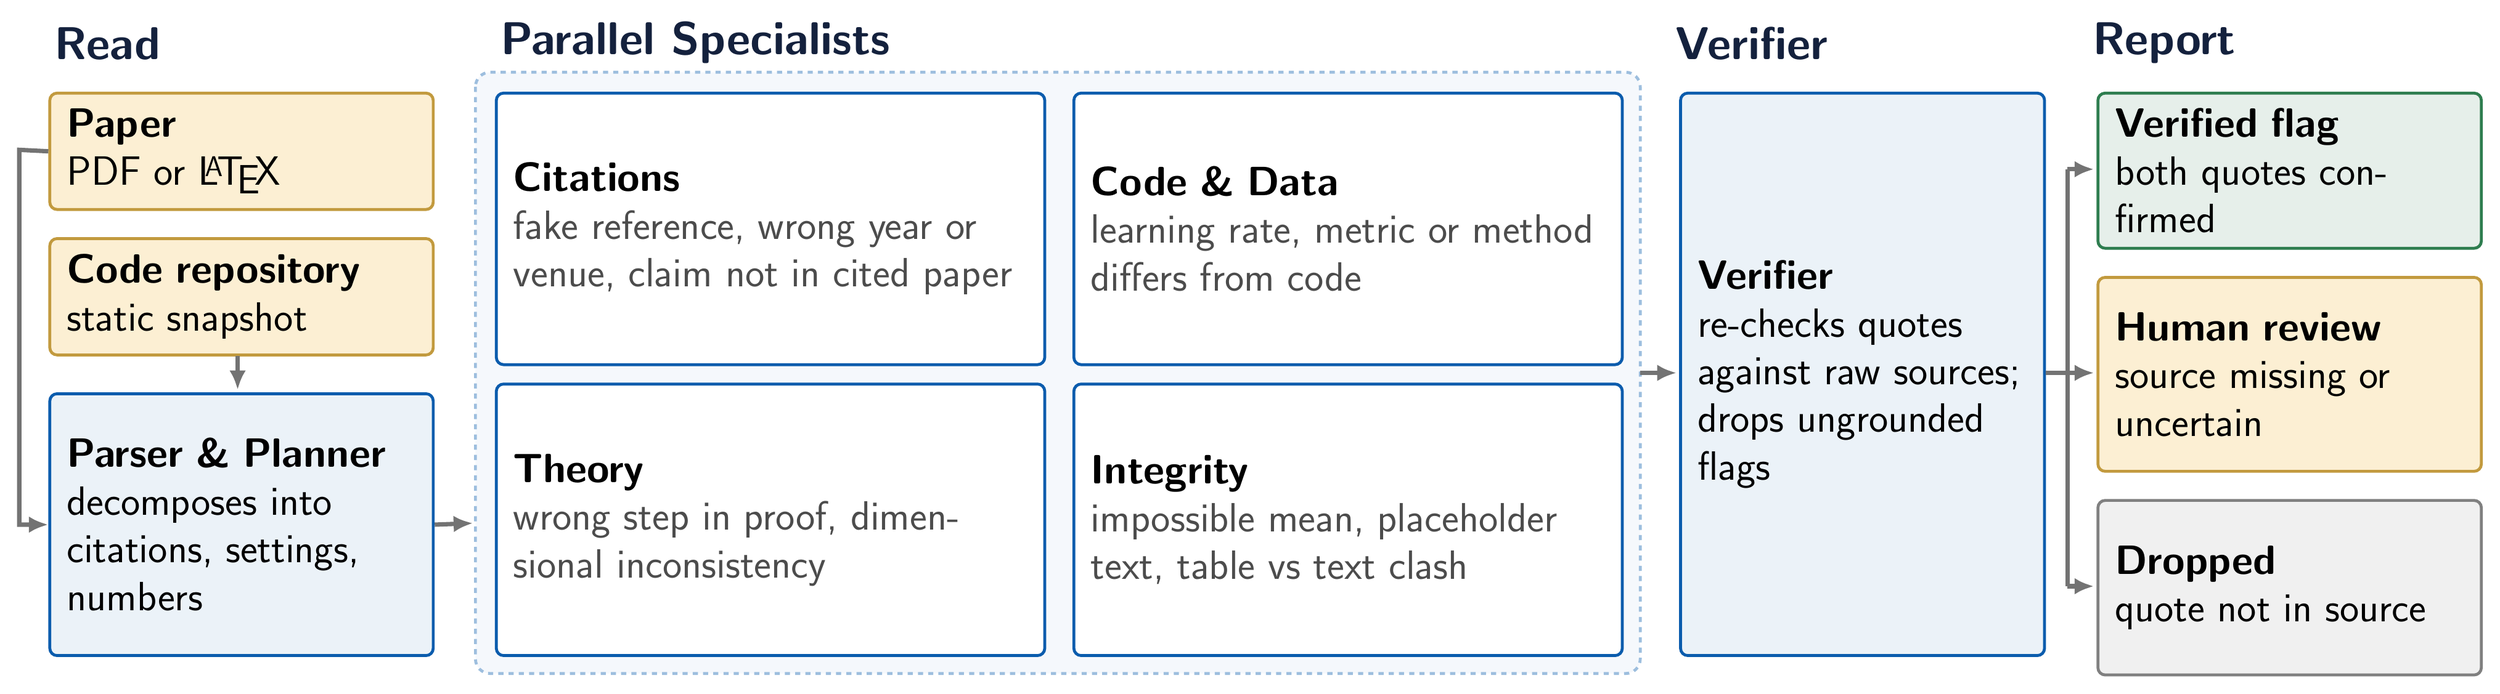
\begin{tikzpicture}[x=1mm, y=1mm, font=\sffamily\fontsize{24}{28}\selectfont,
  bx/.style={draw=#1, line width=0.6mm, rounded corners=1.5mm, align=left, inner xsep=3.5mm,
    inner ysep=2mm, anchor=north west},
  ar/.style={-{Latex[length=4mm,width=3.4mm]}, line width=0.9mm, black!55},
  ln/.style={line width=0.9mm, black!55},
  stitle/.style={anchor=west, font=\sffamily\bfseries\fontsize{27}{31}\selectfont\color{ink}}]
\foreach \x/\n/\s in {0/1/Read, 92/2/Parallel Specialists, 334/3/Verifier, 420/4/Report} {
  \node[stitle] at (\x,10) {\s};
}
\node[bx=crev!80!black, fill=crev!25, text width=72mm, minimum height=24mm] (pdf) at (0,0)
  {\textbf{Paper}\\ PDF or \LaTeX};
\node[bx=crev!80!black, fill=crev!25, text width=72mm, minimum height=24mm] (repo) at (0,-30)
  {\textbf{Code repository}\\ static snapshot};
\node[bx=blue, fill=blue!8, text width=72mm, minimum height=54mm] (parse) at (0,-62)
  {\textbf{Parser \& Planner}\\ decomposes into citations, settings, numbers};
\draw[ar] (39,-54.5) -- (39,-61.5);
\draw[ar] (pdf.west) -- (-6,-12) |- (parse.west);

\fill[blue!4, rounded corners=3mm] (88,4) rectangle (328,-120);
\draw[blue!40, line width=0.6mm, dashed, rounded corners=3mm] (88,4) rectangle (328,-120);
\foreach \x/\y/\name/\what in {
   92/0/Citations/{fake reference, wrong year or venue, claim not in cited paper},
  211/0/Code \& Data/{learning rate, metric or method differs from code},
   92/-60/Theory/{wrong step in proof, dimensional inconsistency},
  211/-60/Integrity/{impossible mean, placeholder text, table vs text clash}} {
  \node[bx=blue, fill=white, text width=106mm, minimum height=56mm] at (\x,\y)
    {\textbf{\name}\\ {\color{black!70}\what}};
}
\draw[ar] (parse.east) -- (87.5,-89);

\node[bx=blue, fill=blue!8, text width=68mm, minimum height=116mm] (ver) at (336,0)
  {\textbf{Verifier}\\ re-checks quotes against raw sources; drops ungrounded flags};
\draw[ar] (328,-58) -- (335.5,-58);

\node[bx=good, fill=good!12, text width=72mm, minimum height=32mm] (ok) at (422,0)
  {\textbf{Verified flag}\\ both quotes confirmed};
\node[bx=crev!80!black, fill=crev!25, text width=72mm, minimum height=40mm] (hum) at (422,-38)
  {\textbf{Human review}\\ source missing or uncertain};
\node[bx=black!50, fill=black!6, text width=72mm, minimum height=36mm] (drop) at (422,-84)
  {\textbf{Dropped}\\ quote not in source};
\draw[ln] (ver.east |- 0,-58) -- (416,-58);
\draw[ln] (416,-16) -- (416,-102);
\foreach \y in {-16,-58,-102} \draw[ar] (416,\y) -- (421.5,\y);
\end{tikzpicture}}\par}

\vspace{1.5mm}
\textbf{Evidence Gate:} Discrepancies lacking exact verbatim quotes are dropped before human review.
\end{col}

\vspace{3mm plus 1fill}

% ================================================================ ROW 2: 3 Columns
% ---------------- COLUMN 1: Benchmark & Engineering Choices
\begin{col}{0.315\linewidth}{r2}
\sect{3}{What we tested on}
\begin{minipage}[t]{0.5\linewidth}\stat{cfull}{40}{papers + code}{with realistic injected errors}\end{minipage}%
\begin{minipage}[t]{0.5\linewidth}\stat{bad}{163}{known errors}{and 72 clean items}\end{minipage}

\vspace{3mm}
\begin{minipage}[t]{0.5\linewidth}\stat{blue}{831}{references}{HALLMARK benchmark}\end{minipage}%
\begin{minipage}[t]{0.5\linewidth}\stat{good}{13}{papers with proofs}{SPOT benchmark}\end{minipage}

\vspace{4mm}
\sect{4}{Ablations: What works}
{\smalltext
\textbf{Finding code for methods}\par\vspace{1mm}
\cbar{Embeddings}{59}{0.702}{cfull}
\cbar{Word overlap}{35}{0.417}{black!30}
{\color{black!60}changed line shown, of 84}\par\vspace{3.5mm}
\textbf{Reading PDF tables}\par\vspace{1mm}
\cbar{Table region}{98\%}{0.98}{cfull}
\cbar{GROBID}{41\%}{0.41}{black!30}
\vspace{2.5mm}
\textbf{Model reading code}\par\vspace{1mm}
\cbar{3.8 Flash}{17, 1$\times$}{0.298}{cfull}
\cbar{3.1 Pro}{19, 3.6$\times$}{0.333}{black!30}
{\color{black!60}changes found of 57, and cost}\par\vspace{2.5mm}
\textbf{Deterministic rules:} 100\% catch on formatting and sanity checks with \$0 cost.\par\vspace{1.5mm}
{\color{cfull}\rule{4mm}{4mm}} what we kept\par}
\end{col}\hfill
% ---------------- COLUMN 2: Headline Results & Comparison
\begin{col}{0.335\linewidth}{r2}
\sect{5}{Results: 13$\times$ over baselines}
\begin{minipage}[t]{0.5\linewidth}\stat{cfull}{0.636}{Macro-F1}{baselines: 0.05}\end{minipage}%
\begin{minipage}[t]{0.5\linewidth}\stat{good}{0}{false alarms}{on 72 clean items}\end{minipage}

\vspace{3mm}
\begin{minipage}[t]{0.5\linewidth}\stat{blue}{100\%}{flags with quote}{baselines: 0\%}\end{minipage}%
\begin{minipage}[t]{0.5\linewidth}\stat{ink}{\rs7.4}{per paper}{B1 (Agent): \rs51}\end{minipage}

\vspace{4mm}
\sect{6}{Finds what an LLM misses}
{\centering
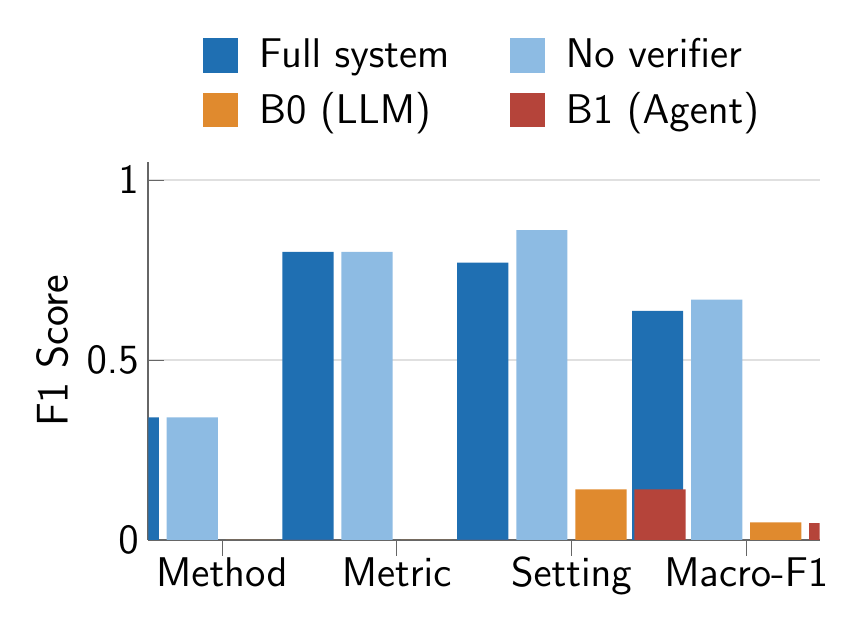
\begin{tikzpicture}
\begin{axis}[poster, width=\linewidth-36mm, height=48mm, scale only axis,
  ybar=1mm, bar width=6.5mm, ymin=0, ymax=1.05,
  symbolic x coords={Method,Metric,Setting,Macro-F1}, xtick=data,
  enlarge x limits=0.14, ytick={0,0.5,1}, ylabel={F1 Score},
  legend image code/.code={\fill[#1] (0mm,-2.2mm) rectangle (4.4mm,2.2mm);},
  legend style={at={(0.5,1.06)}, anchor=south, legend columns=2, draw=none, fill=none,
    font=\fontsize{15}{18}\selectfont, cells={anchor=west}, row sep=1.2mm,
    /tikz/every odd column/.append style={column sep=2mm},
    /tikz/every even column/.append style={column sep=7mm}},
  ymajorgrids, axis x line*=bottom, axis y line*=left]
\addplot[fill=cfull,draw=none] coordinates {(Method,0.34) (Metric,0.80) (Setting,0.77) (Macro-F1,0.636)};
\addplot[fill=cnover,draw=none] coordinates {(Method,0.34) (Metric,0.80) (Setting,0.86) (Macro-F1,0.667)};
\addplot[fill=cbzero,draw=none] coordinates {(Method,0) (Metric,0) (Setting,0.14) (Macro-F1,0.048)};
\addplot[fill=cbone,draw=none] coordinates {(Method,0) (Metric,0) (Setting,0.14) (Macro-F1,0.046)};
\legend{Full system, No verifier, B0 (LLM), B1 (Agent)}
\end{axis}
\end{tikzpicture}\par}

\vspace{2.5mm}
We aimed for 10 points above baselines and got \hlmark{59 F1 points}.\\[1mm]
{\smalltext Neither LLM baseline finds a single method or metric error; our modular pipeline achieves \textbf{0.80 F1 on Metric} and \textbf{0.77 F1 on Setting}.\par}
\end{col}\hfill
% ---------------- COLUMN 3: Verifier Impact & Web App
\begin{col}{0.325\linewidth}{r2}
\sect{7}{Specialist accuracy \& fewer flags}
{\centering
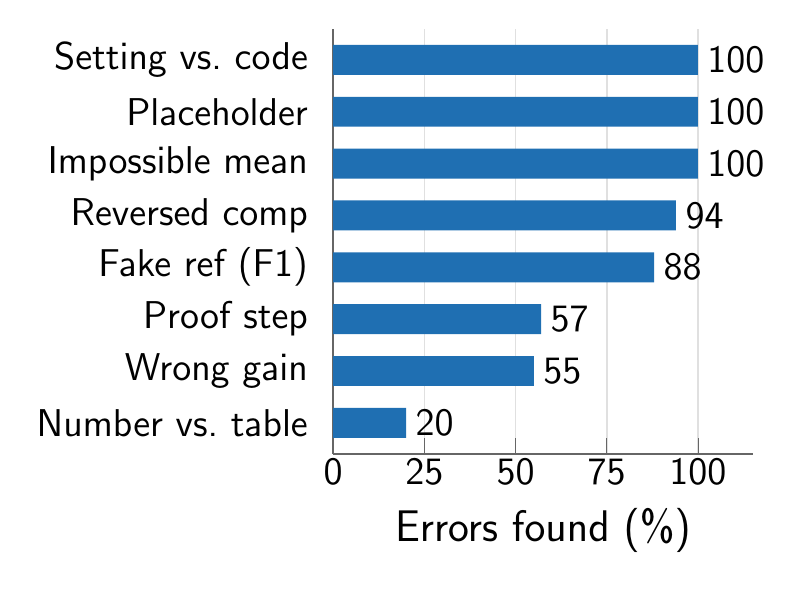
\begin{tikzpicture}
\begin{axis}[poster, width=\linewidth-68mm, height=54mm, scale only axis,
  xbar, bar width=3.8mm, bar shift=0pt, xmin=0, xmax=115, every tick label/.append style={font=\fontsize{14}{17}\selectfont}, ymin=0.4, ymax=8.6,
  ytick={1,...,8}, yticklabels={Number vs.\ table, Wrong gain, Proof step, Fake ref (F1),
    Reversed comp, Impossible mean, Placeholder, Setting vs.\ code},
  xtick={0,25,50,75,100}, xlabel={Errors found (\%)}, axis x line*=bottom, axis y line*=left,
  ytick style={draw=none}, xmajorgrids,
  nodes near coords, every node near coord/.append style={anchor=west,
    font=\sffamily\fontsize{14}{17}\selectfont\bfseries}]
\addplot[fill=cfull,draw=none] coordinates {(20,1) (55,2) (57,3) (88,4) (94,5) (100,6) (100,7) (100,8)};
\end{axis}
\end{tikzpicture}\par}

\vspace{1.5mm}
{\smalltext Rule checks catch \textbf{100\%} of planted placeholders and impossible means. Verifier drops \hlmark{35\% spurious flags} (391 $\to$ 255 flags to review).\par}

\vspace{3mm}
\sect{8}{Cheaper \& Interactive Web App}
\begin{minipage}[c]{0.48\linewidth}
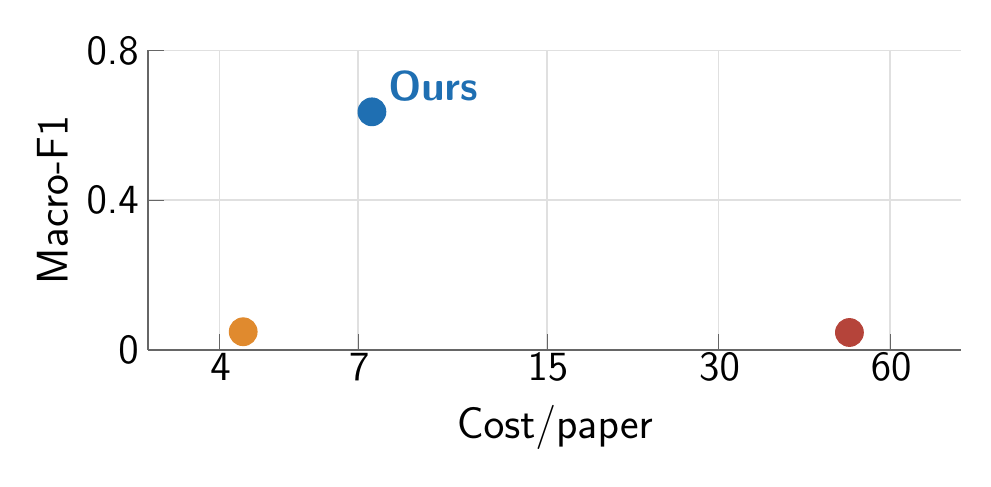
\begin{tikzpicture}
\begin{semilogxaxis}[poster, width=\linewidth-18mm, height=38mm, scale only axis,
  xmin=3, xmax=80, ymin=0, ymax=0.8,
  xtick={4,7,15,30,60}, xticklabels={\rs4,\rs7,\rs15,\rs30,\rs60},
  ytick={0,0.4,0.8},
  xlabel={Cost/paper}, ylabel={Macro-F1},
  grid=major, axis x line*=bottom, axis y line*=left]
\addplot[only marks, mark=*, mark size=5pt, cfull] coordinates {(7.4,0.636)};
\addplot[only marks, mark=*, mark size=5pt, cbzero] coordinates {(4.4,0.048)};
\addplot[only marks, mark=*, mark size=5pt, cbone] coordinates {(50.9,0.046)};
\node[anchor=south west, font=\fontsize{15}{18}\selectfont\bfseries\color{cfull}] at (axis cs:7.6,0.64) {Ours};
\end{semilogxaxis}
\end{tikzpicture}
\end{minipage}\hfill
\begin{minipage}[c]{0.50\linewidth}
\setlength{\fboxsep}{0pt}\setlength{\fboxrule}{0.5mm}%
\fcolorbox{rulegrey}{white}{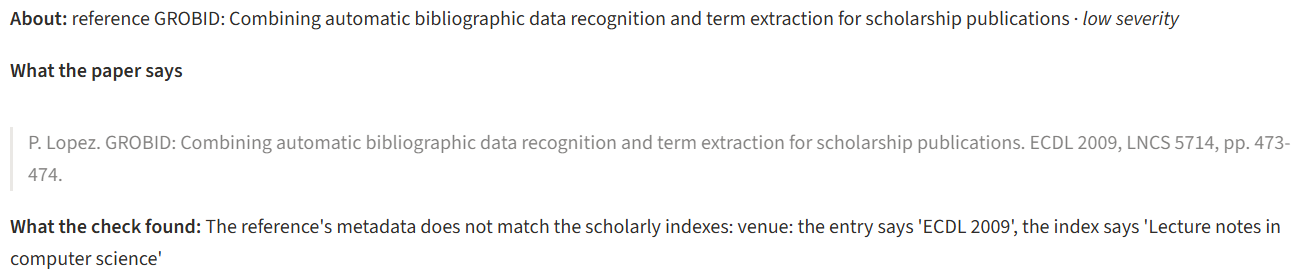
\includegraphics[width=\linewidth]{../app_screenshots/light_claim.png}}\\[1mm]
{\smalltext\centering Dual verbatim quotes in UI\par}
\end{minipage}

\vspace{1.5mm}
Ours costs \textbf{\rs7.4} vs B1 (Agent) \hlmark{\rs51} (7$\times$ cheaper, 13$\times$ more accurate). Live Streamlit interface tracks budget and triage decisions.
\end{col}

\vspace{2mm plus 1fill}

% ================================================================ FOOTER (Affiliations, 5 Key References & QR Codes)
\begin{minipage}[b]{0.63\linewidth}
  {\fontsize{16}{20}\selectfont\color{black!80}\textbf{SERC} \& \textbf{CVIT}, International Institute of Information Technology, Hyderabad (IIIT-H)}\\[1.5mm]
  {\fontsize{13.5}{17}\selectfont\color{ink}\textbf{Key References:}\enspace
  \textbf{[1]} Kim et al., \emph{HALLMARK: Diagnosing LLM citation verifiers}, arXiv 2026.\enspace
  \textbf{[2]} Baumg\"artner \& Gurevych, \emph{SciCoQA: Paper--code alignment}, arXiv 2026.\enspace
  \textbf{[3]} Son et al., \emph{SPOT: Automated scientific verification}, arXiv 2025.\enspace
  \textbf{[4]} Yao et al., \emph{ReAct: Synergizing reasoning and acting}, ICLR 2023.\enspace
  \textbf{[5]} Lopez, \emph{GROBID: Bibliographic data recognition}, ECDL 2009.}
\end{minipage}\hfill
\begin{minipage}[b]{0.35\linewidth}\raggedleft
  {\fontsize{18}{22}\selectfont\bfseries\color{ink}\faGithub\ Code}\enspace
  \raisebox{-1.5mm}{\qrcode[height=21mm]{\codeurl}}\hspace{9mm}%
  {\fontsize{18}{22}\selectfont\bfseries\color{ink}\faGlobe\ Website}\enspace
  \raisebox{-1.5mm}{\qrcode[height=21mm]{\websiteurl}}
\end{minipage}

\end{document}
